% Options for packages loaded elsewhere
\PassOptionsToPackage{unicode}{hyperref}
\PassOptionsToPackage{hyphens}{url}
%
\documentclass[
]{article}
\usepackage{amsmath,amssymb}
\usepackage{iftex}
\ifPDFTeX
  \usepackage[T1]{fontenc}
  \usepackage[utf8]{inputenc}
  \usepackage{textcomp} % provide euro and other symbols
\else % if luatex or xetex
  \usepackage{unicode-math} % this also loads fontspec
  \defaultfontfeatures{Scale=MatchLowercase}
  \defaultfontfeatures[\rmfamily]{Ligatures=TeX,Scale=1}
\fi
\usepackage{lmodern}
\ifPDFTeX\else
  % xetex/luatex font selection
\fi
% Use upquote if available, for straight quotes in verbatim environments
\IfFileExists{upquote.sty}{\usepackage{upquote}}{}
\IfFileExists{microtype.sty}{% use microtype if available
  \usepackage[]{microtype}
  \UseMicrotypeSet[protrusion]{basicmath} % disable protrusion for tt fonts
}{}
\makeatletter
\@ifundefined{KOMAClassName}{% if non-KOMA class
  \IfFileExists{parskip.sty}{%
    \usepackage{parskip}
  }{% else
    \setlength{\parindent}{0pt}
    \setlength{\parskip}{6pt plus 2pt minus 1pt}}
}{% if KOMA class
  \KOMAoptions{parskip=half}}
\makeatother
\usepackage{xcolor}
\usepackage[margin=1in]{geometry}
\usepackage{graphicx}
\makeatletter
\def\maxwidth{\ifdim\Gin@nat@width>\linewidth\linewidth\else\Gin@nat@width\fi}
\def\maxheight{\ifdim\Gin@nat@height>\textheight\textheight\else\Gin@nat@height\fi}
\makeatother
% Scale images if necessary, so that they will not overflow the page
% margins by default, and it is still possible to overwrite the defaults
% using explicit options in \includegraphics[width, height, ...]{}
\setkeys{Gin}{width=\maxwidth,height=\maxheight,keepaspectratio}
% Set default figure placement to htbp
\makeatletter
\def\fps@figure{htbp}
\makeatother
\setlength{\emergencystretch}{3em} % prevent overfull lines
\providecommand{\tightlist}{%
  \setlength{\itemsep}{0pt}\setlength{\parskip}{0pt}}
\setcounter{secnumdepth}{5}
\usepackage[german]{babel}
\usepackage{mathtools}
\usepackage{tikz}
\usepackage{pgf}
\usepackage{csquotes}
\AtBeginDocument{
\renewcommand{\maketitle}{}
}
\PassOptionsToPackage{a4paper,margin = 2.5cm}{geometry}
\usepackage{geometry}
\newcommand{\bcenter}{\begin{center}}
\newcommand{\ecenter}{\end{center}}
\renewcommand{\contentsname}{Inhalt}
\usepackage{blindtext}
\usepackage[backend=biber, style = apa]{biblatex}
\addbibresource{Literatur.bib}
\usepackage{multirow}
\usepackage{booktabs}
\usepackage{array}
\usepackage{pdflscape}
\ifLuaTeX
  \usepackage{selnolig}  % disable illegal ligatures
\fi
\usepackage[]{biblatex}
\addbibresource{Literatur.bib}
\IfFileExists{bookmark.sty}{\usepackage{bookmark}}{\usepackage{hyperref}}
\IfFileExists{xurl.sty}{\usepackage{xurl}}{} % add URL line breaks if available
\urlstyle{same}
\hypersetup{
  pdftitle={Ergebnisse},
  pdfauthor={Franz Andersch \& Niklas Münz},
  hidelinks,
  pdfcreator={LaTeX via pandoc}}

\title{Ergebnisse}
\author{Franz Andersch \& Niklas Münz}
\date{2024-08-22}

\begin{document}
\maketitle

\subsection{Vorgehensweise bei der Analyse}

Bevor die Ergebnisse erläutert werden, wird kurz auf die Vorgehensweise
bei der Analyse eingegangen. In die Analyse werden fünf Modelle
einbezogen: SVM mit linearem, polynomialem und radialem Kern, sowie
regularisierte logistische Regression und k-nearest neighbours.\newline
Vor dem erstellen der Modelle wird ein Tuning der Hyperparameter je
Modell durchgeführt. Dafür wird die Bayesian Optimization Methode
genutzt, welche ein iterativer Algorithmus ist. Hierbei werden die
nächsten Evaluierungspunkte basierend auf zuvor beobachteten Ergebnissen
bestimmt \parencite{yangHyperparameterOptimizationMachine2020}. Der
Algorithmus basiert auf zwei Hauptkomponenten: einem Surrogatmodell und
einer Akqusitionsfunktion. Das Surrogatmodell, wofür hier ein Gaussian
Process genutzt wird, passt die bisher beobachteten Punkte an die
Zielfunktion an. Die Akquisitionsfunktion wählt dann die nächsten Punkte
aus, wobei ein Gleichgewicht zwischen der Erkundung neuer Bereiche und
der Nutzung vielversprechender Regionen angestrebt wird. Dafür wird hier
der Ansatz des Upper-Confidence-Bound genutzt, welcher obere
Konfidenzgrenzen nutzt um den Verlust gegenüber der besten möglichen
Entscheidung, während der Optimierung zu minimieren
\parencite{snoekPracticalBayesianOptimization2012}. \begin{align}
a_{UCB}(\mathbf{x};~\left\{\mathbf{x}_n,y_n\right\},\theta) = \mu(\mathbf{x};~\left\{\mathbf{x}_n,y_n\right\},\theta) - k \sigma(\mathbf{x};~\left\{\mathbf{x}_n,y_n\right\},\theta)
\end{align} Die Bayesian Optimization wird genutzt, da sie eine schnelle
Konvergenz für stetige Hyperparameter aufweist
\parencite{yangHyperparameterOptimizationMachine2020}. Als
Evaluierungskriterium wird die Genauigkeit der Modelle, welche durch den
Anteil der korrekt klassifizierten Beobachtungen wiedergegeben wird,
verwendet.

Basierend auf den Ergebnissen des Tuning werden die oben genannten
Modelle erstellt. Daraufhin werden die Genauigkeit, die Receiver
Operating Characteristic Kurve (ROC-Kurve) bzw. der Area Under The Curve
Wert (AUC-Wert) und der F1-Score für jedes Modell bestimmt.\newline Die
ROC-Kurve ist eine grafische Darstellung der Leistungsfähigkeit eines
Klassifikationsmodells, wobei die Sensitivität auf der y-Achse von 0 bis
1 gegen die Spezifität auf der x-Achse von 1 bis 0 abgetragen wird
\parencite{fawcettIntroductionROCAnalysis2006}. Sensitivität und
Spezifität ergeben sich aus: \begin{align}
Sensitivität=\frac{korrekt~Positiv}{korrekt~Positiv~+~falsch~Negativ}
\end{align} \begin{align}
Spezifität=\frac{korrekt~Negativ}{falsch~Positiv~+~korrekt~Negativ}
\end{align} Positiv ist in diesem Fall gleichbedeutend mit Klasse 1 und
Negativ mit Klasse 2. Die ROC-Kurve zeigt dann den Zusammenhang zwischen
dem Nutzen (korrekt Positive) und den Kosten (falsch Positive) auf. Eine
ideale Kurve läuft nah am linken, oberen Rand der Grafik, da hier
bereits bei sehr hoher Spezifität (hohe Anzahl korrekt Negative) eine
hohe Sensitivität (hohe Anzahl korrekt Positive) erreicht wird. Der
AUC-Wert bezieht sich auf die Fläche unterhalb der Kurve und liegt somit
im Intervall {[}0,1{]}, wobei ein Wert von 1 für eine perfekte
Klassifikation spricht, während ein Wert von 0.5 glechbedeutend mit
einer rein zufälligen Zuordnung der Klassen spricht.\newline Für den
F1-Score ist außerdem die Präzision von Bedeutung, die sich wie folgt
berechnet\parencite{fawcettIntroductionROCAnalysis2006}: \begin{align}
Präzision=\frac{korrekt~Positiv}{korrekt~Positiv~+~falsch~Positiv}
\end{align} Der F1-Score beschreibt das harmonische Mittel zwischen
Präzision und Sensitivität und drückt folglich die Fähigkeit des
Modells, gleichzeitig falsch Positive und falsch Negative zu minimieren,
aus. \begin{align}
F1\text{-}Score=\frac{2}{1/Präzision~+~1/Sensitivität}
\end{align}\newline Zuletzt wird innerhalb jeder Datensituation, für
jeden Algorithmus ein Rang vergeben, der sich aus der Summe der drei
Auswertungskriterien Genauigkeit, AUC-Wert sowie F1-Score ergibt. Dabei
steht Rang 1 für den am besten abschneidenden Algorithmus in der
jeweiligen Datensituation.

\subsection{Darstellung der Ergebnisse}

Tabelle 2 zeigt die Leistungsfähigkeit der fünf
Klassifikationsalgorithmen über die neun verschiedenen Datensituationen
anhand drei verschiedener Evaluationskriterien, sowie den Rang in der
jeweiligen Datensituation.\newline

\begin{landscape}

\begin{table}[h] \centering \begin{tabular}{|c|c|c|c|} \hline
 & \textbf{linear} & \textbf{polynomial} & \textbf{radial} \\ \hline \multirow{5}{*}{\textbf{$p \ll n$}} &  
\begin{tabular}{lrrrr}
\toprule
  & ACC & AUC & F1 & Rang\\
\midrule
SVM-L & 0.956 & 0.991 & 0.956 & 4\\
SVM-P & 0.956 & 0.991 & 0.956 & 3\\
SVM-R & 0.961 & 0.991 & 0.961 & 1\\
LogR & 0.957 & 0.992 & 0.957 & 2\\
K-NN & 0.582 & 0.599 & 0.582 & 5\\
\bottomrule
\end{tabular}  &  
\begin{tabular}{lrrrr}
\toprule
  & ACC & AUC & F1 & Rang\\
\midrule
SVM-L & 0.665 & 0.728 & 0.659 & 5\\
SVM-P & 0.674 & 0.729 & 0.671 & 4\\
SVM-R & 0.704 & 0.759 & 0.690 & 1\\
LogR & 0.687 & 0.740 & 0.687 & 2\\
K-NN & 0.691 & 0.731 & 0.657 & 3\\
\bottomrule
\end{tabular}  &  
\begin{tabular}{lrrrr}
\toprule
  & ACC & AUC & F1 & Rang\\
\midrule
SVM-L & 0.525 & 0.532 & 0.620 & 4\\
SVM-P & 1.000 & 1.000 & 1.000 & 1\\
SVM-R & 0.913 & 0.994 & 0.905 & 3\\
LogR & 0.506 & 0.530 & 0.532 & 5\\
K-NN & 0.978 & 0.978 & 0.978 & 2\\
\bottomrule
\end{tabular}  \\ \hline \multirow{5}{*}{\textbf{$p \approx n$}} &  
\begin{tabular}{lrrrr}
\toprule
  & ACC & AUC & F1 & Rang\\
\midrule
SVM-L & 0.82 & 0.869 & 0.816 & 3\\
SVM-P & 0.82 & 0.869 & 0.816 & 3\\
SVM-R & 0.86 & 0.875 & 0.844 & 2\\
LogR & 0.88 & 0.918 & 0.864 & 1\\
K-NN & 0.66 & 0.622 & 0.667 & 5\\
\bottomrule
\end{tabular}  &  
\begin{tabular}{lrrrr}
\toprule
  & ACC & AUC & F1 & Rang\\
\midrule
SVM-L & 0.50 & 0.504 & 0.545 & 4\\
SVM-P & 0.58 & 0.525 & 0.571 & 3\\
SVM-R & 0.56 & 0.530 & 0.389 & 5\\
LogR & 0.64 & 0.563 & 0.667 & 1\\
K-NN & 0.56 & 0.552 & 0.577 & 2\\
\bottomrule
\end{tabular}  &  
\begin{tabular}{lrrrr}
\toprule
  & ACC & AUC & F1 & Rang\\
\midrule
SVM-L & 0.68 & 0.605 & 0.724 & 4\\
SVM-P & 0.84 & 0.912 & 0.852 & 1\\
SVM-R & 0.84 & 0.886 & 0.818 & 2\\
LogR & 0.64 & 0.526 & 0.690 & 5\\
K-NN & 0.80 & 0.800 & 0.833 & 3\\
\bottomrule
\end{tabular}  \\ \hline \multirow{5}{*}{\textbf{$p \gg n$}} &  
\begin{tabular}{lrrrr}
\toprule
  & ACC & AUC & F1 & Rang\\
\midrule
SVM-L & 0.72 & 0.786 & 0.708 & 3\\
SVM-P & 0.74 & 0.792 & 0.735 & 2\\
SVM-R & 0.54 & 0.500 & 0.439 & 5\\
LogR & 0.80 & 0.814 & 0.808 & 1\\
K-NN & 0.62 & 0.584 & 0.513 & 4\\
\bottomrule
\end{tabular}  &  
\begin{tabular}{lrrrr}
\toprule
  & ACC & AUC & F1 & Rang\\
\midrule
SVM-L & 0.62 & 0.574 & 0.612 & 1\\
SVM-P & 0.62 & 0.574 & 0.612 & 1\\
SVM-R & 0.50 & 0.500 & NaN & 5\\
LogR & 0.60 & 0.562 & 0.600 & 3\\
K-NN & 0.50 & 0.612 & 0.490 & 4\\
\bottomrule
\end{tabular}  &  
\begin{tabular}{lrrrr}
\toprule
  & ACC & AUC & F1 & Rang\\
\midrule
SVM-L & 0.56 & 0.504 & 0.633 & 5\\
SVM-P & 0.72 & 0.882 & 0.774 & 2\\
SVM-R & 0.72 & 0.744 & 0.611 & 3\\
LogR & 0.58 & 0.530 & 0.656 & 4\\
K-NN & 0.88 & 0.880 & 0.893 & 1\\
\bottomrule
\end{tabular}  \\ \hline \end{tabular} \caption{Vergleich der Modelle} \end{table}

\end{landscape}

In den Datensituationen mit linearer Form der Entscheidungsgrenze
performt insbesondere \(logR\) gut, da sie in allen drei Szenarien über
alle Kriterien hinweg einen Wert von mindestens 0.8 aufweist und jeweils
mindestens Rang 2 belegt. Im Falle von \(p \ll n\) und \(p \approx n\)
zeigen auch \(SVM-L\), \(SVM-P\) und \(SVM-R\) eine gute Leistung mit
Werten um 0.9. In dem hochdimensionalen Setting \(p \gg n\) ist die
Performance jedoch differnzierter zu betrachten. Hier schneiden
\(SVM-L\) und \(SVM-P\) nach wie vor ordentlich ab. \(SVM-R\) zeigt hier
jedoch deutliche Defizite über alle Kriterien hinweg mit Werten um 0.5.
\(K-NN\) schneidet im linearen Kontext über alle Szenarien hinweg
schlecht ab, wobei die Genauigkeit maximal bei 0.66 im Falle von
\(p \approx n\) liegt.\newline Die ROC-Kurven werden nur in den
Datensituationen mit \(p \ll n\) genutzt, da die grafische Darstellung
in Szenarien mit kleinem \(n\) nicht sinnvoll erscheint. Abbildung 8
zeigt die ROC-Kurven für die Datensituation S1. Diese zeigt grafisch
noch einmal den deutlichen Unterschied zwischen \(K-NN\), welcher nur
etwas besser als eine reine Zufallsauswahl ist und den anderen vier
Algorithmen, welche nahezu perfekt klassifizieren.

\begin{figure}
\centering
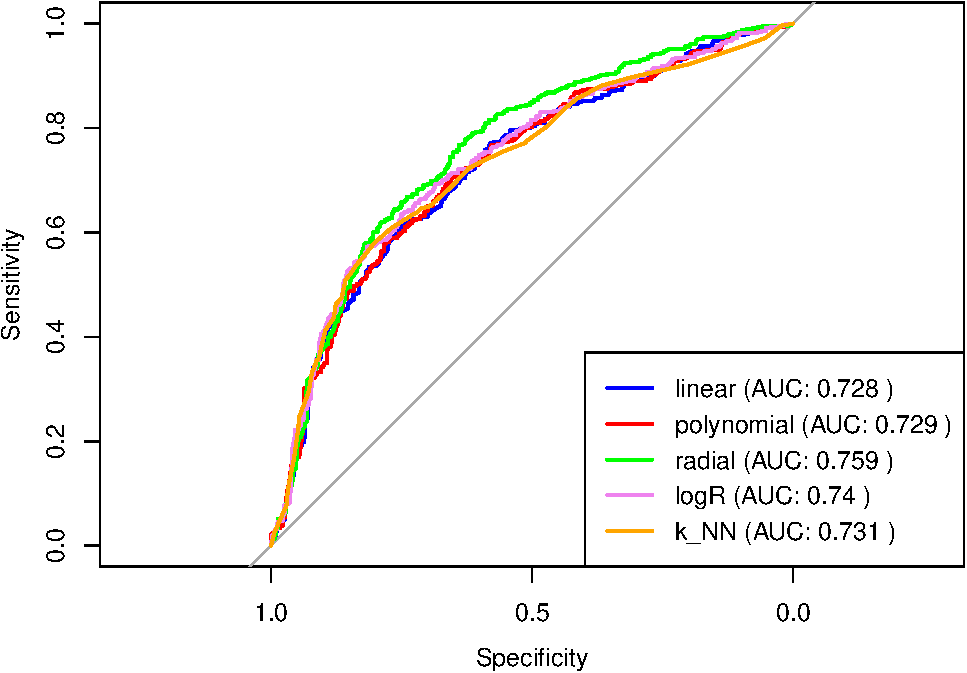
\includegraphics{Ergebnisse_files/figure-latex/unnamed-chunk-2-1.pdf}
\caption{ROC-Kurven Szenario 1}
\end{figure}

In den Datensituationen mit polynomialer Form der Entscheidungsgrenze
ist die Leistungsfähigkeit aller Algorithmen grundsätzlich deutlich
schlechter als in den zuvor beschriebenen Szenarien. Im Fall von
\(p \ll n\) sind die Ergebnisse mittelmäßig mit Werten um 0.7, wobei
sich kein Algorithmus von den anderen absetzen kann. Bei \(p \approx n\)
ist \(LogR\) den anderen Klassifikationsmethoden leicht überlegen,
insbesondere bei der Fähigkeit gleichzeitig falsch Positive und falsch
Negative zu minimieren (F1-Score = 0.667). Die anderen Algorithmen
befinden sich durchweg über alle Werte hinweg nahe 0.5. Ähnlich ist es
der Fall für \(p \gg n\) bei dem nun \(SVM-L\), \(SVM-P\) und \(LogR\)
mit einer Genauigkeit von 0.6, \(SVM-R\) und \(K-NN\) mit einer
Genauigkeit von 0.5 leicht überlegen sind. Dennoch ist für die letzten
beiden Szenarien deutlich, dass kein Algorithmus gute Leistung
zeigt.\newline Abbildung 9 zeigt die ROC-Kurven für Szenario 2. Hieraus
wird erneut deutlich, dass sich kein Algorithmus von den anderen abheben
kann, wobei alle eine mittelmäßige Leistung zeigen.

\begin{figure}
\centering
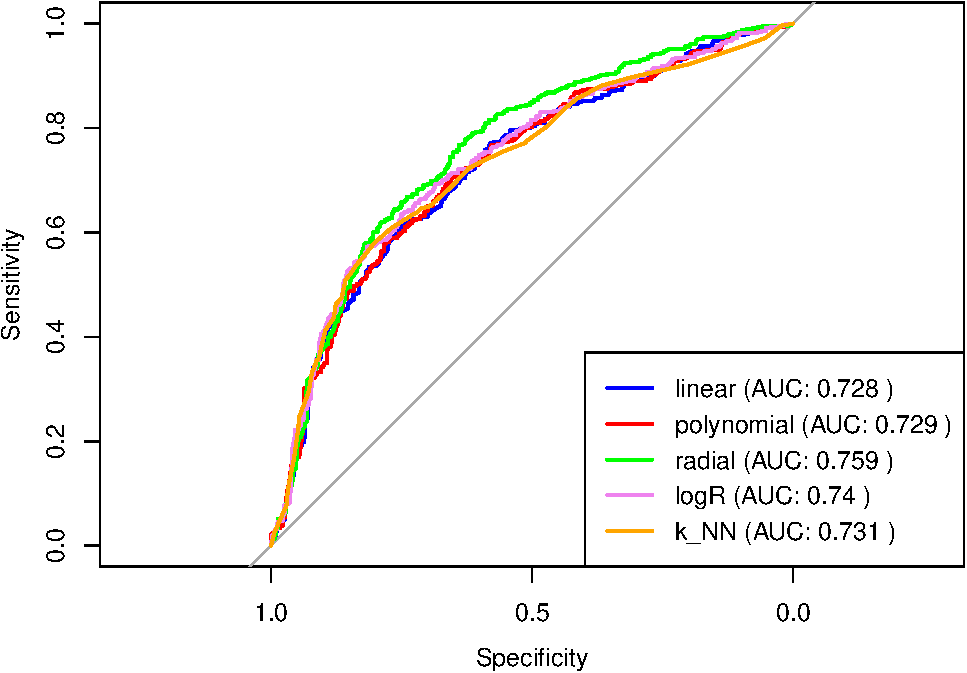
\includegraphics{Ergebnisse_files/figure-latex/unnamed-chunk-3-1.pdf}
\caption{ROC-Kurven Szenario 2}
\end{figure}

In den Datensituationen mit radialer Form der Entscheidungsgrenze ist
für den Fall \(p \ll n\) eine eindeutige Unterscheidung zu treffen.
Während \(SVM-P\), \(SVM-R\) und \(K-NN\) (nahezu) perfekt
klassifizieren, haben dabei \(SVM-L\) und \(LogR\) große Probleme und
zeigen lediglich Werte nahe 0.5. Weniger drastisch aber dennoch mit dem
gleichen Resultat ist dies für \(p \approx n\) der Fall. Während
\(SVM-P\), \(SVM-R\) und \(K-NN\) etwas schlechter abschneiden
(beispielsweise mit F1-Scores zwischen 0.8 und 0.9), performen \(SVM-L\)
und \(LogR\) leicht besser (beispielsweise mit F1-Scores nahe 0.7).
Innerhalb dieser beiden Gruppen gibt es keine nennenswerten
Unterschiede. Für \(p \gg n\) sind ebenfalls die beiden Gruppen zu
differenzieren. Für \(SVM-L\) und \(LogR\) sind wie in Szenario 3 wieder
Werte nahe 0.5 bzw. nahe 0.6 für die F1-Scores erkennbar. \(SVM-P\) und
\(SVM-R\) performen in diesem Szenario am schlechtesten, wobei die
AUC-Werte von 0.882 bzw. 0.744 weiterhin akzeptable Leistungen zeigen.
Heraus sticht \(K-NN\), insbesondere bei dem F1-Score von 0.893, was
verdeutlicht das dieser Algorithmus hier die beste Leistung
zeigt.\newline Abbildung 10 zeigt die ROC-Kurven für Szenario 3. Hieraus
wird die Aufteilung in die zwei Gruppen sofort deutlich. \(SVM-P\),
\(SVM-R\) und \(K-NN\) bewegen sich nahe an der oberen linken Kante, was
für eine (nahezu) perfekte Klassifikation spricht. \(SVM-L\) und
\(LogR\) orientieren sich nahe der diagonalen Linie, die eine ROC-Kurve
einer reinen Zufallsauswahl beschreibt. Dies zeigt auf, dass sie kaum
Fähigkeit aufweisen zwischen den Klassen zu unterscheiden.

\begin{figure}
\centering
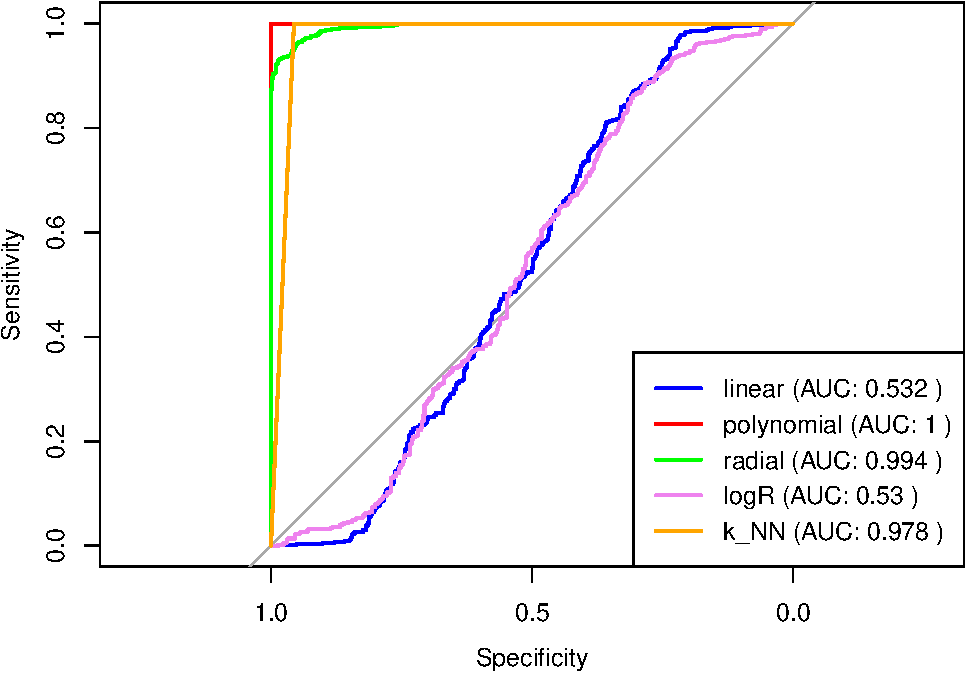
\includegraphics{Ergebnisse_files/figure-latex/unnamed-chunk-4-1.pdf}
\caption{ROC-Kurven Szenario 3}
\end{figure}

Zuletzt wird ein Vergleich der einzelnen Dimensionen über die drei
Formen der Entscheidungsgrenze gezogen. So ist für \(p \ll n\)
ersichtlich, dass insbesondere \(SVM-P\) und \(SVM-R\) über alle drei
Szenarien gute Leistung (insbesondere für S1 und S3 mit mindestens 0.9
über alle Werte) zeigen. Das gleiche gilt, mit Ausnahme der polynomialen
Form der Entscheidungsgrenze, auch für \(p \approx n\), wobei die Werte
etwas niedriger bei 0.8 bis 0.9 liegen. In den hochdimensionalen
Szenarien \(p \gg n\) ist einzig \(SVM-P\) überzeugend, erneut
ausgenommen der polynomialen Form der Entscheidungsgrenze.

\printbibliography

\end{document}
